\documentclass[tikz,border=5pt]{standalone}
\usepackage[UTF8]{ctex}
\usepackage{amsmath,amssymb}
\usetikzlibrary{arrows.meta,calc,angles,quotes,decorations.pathmorphing,patterns}
\definecolor{ink}{HTML}{243447}\definecolor{blue}{HTML}{2765A2}
\definecolor{green}{HTML}{3F7D5B}\definecolor{red}{HTML}{B74739}
\tikzset{body/.style={draw=ink,thick},vec/.style={draw=blue,thick,-{Latex}},guide/.style={gray!60,dashed},dim/.style={ink,{Latex}-{Latex}},line cap=round,line join=round}
\begin{document}

\begin{tikzpicture}
\coordinate(F)at(0,0);\coordinate(D)at(4,0);\coordinate(E)at(2,3.464);
\coordinate(A)at(1,1.732);\coordinate(B)at(2,0);\coordinate(C)at(3,1.732);
\draw[body](F)--(D)--(E)--cycle;
\draw[dim](0,-.6)--node[below]{$2l$}(4,-.6);
\draw[blue,thick](A)--(B)--(C)--cycle;
\foreach\P/\pos in{F/below left,D/below right,E/above,A/left,B/below,C/right}
 \filldraw[fill=white,draw=ink](\P)circle(.06)node[text=ink,\pos]{$\P$};
\node[above,blue]at(2,1.8){闭合弹簧绳：$L_0=3l,\ k$};
\node[below]at(2,-1.2){水平面内俯视；三个小环质量均为 $m$};
\end{tikzpicture}
\begin{tikzpicture}
\coordinate(F)at(0,0);\coordinate(D)at(4,0);\coordinate(E)at(1.5,2.5);
\coordinate(B)at(1.5,0);\coordinate(A)at(1.05882,1.76471);\coordinate(C)at(2,2);
\coordinate(Bone)at(-.705882,1.323529);\coordinate(Btwo)at(4,2.5);
\draw[body](F)--(D)--(E)--cycle;
\draw[guide](D)--(A);\draw[guide](F)--(C);\draw[guide](E)--(B);
\draw[red,thick](A)--(B)--(C);
\draw[green,very thick](Bone)--(Btwo);
\foreach\P/\pos in{F/below left,D/below right,E/above,A/above left,C/above right}
 \fill[ink](\P)circle(2pt)node[\pos]{$\P$};
\fill[ink](B)circle(2pt)node[below]{$B=H$};
\fill[green](Bone)circle(2pt)node[above left]{$B_1$};
\fill[green](Btwo)circle(2pt)node[above right]{$B_2$};
\pic[draw=gray,angle radius=5pt]{right angle=D--A--E};
\pic[draw=gray,angle radius=5pt]{right angle=F--C--D};
\pic[draw=gray,angle radius=5pt]{right angle=E--B--D};
\node[below,align=center]at(1.7,-.7){$B_1$：$B$ 关于 $EF$ 的反射\\$B_2$：$B$ 关于 $ED$ 的反射};
\end{tikzpicture}
\begin{tikzpicture}
\coordinate(F)at(0,0);\coordinate(D)at(4,0);\coordinate(E)at(2,3.464);
\coordinate(A)at(1,1.732);\coordinate(B)at(2,0);
\coordinate(Co)at(3,1.732);\coordinate(C)at(3.35,1.126);
\draw[body](F)--(D)--(E)--cycle;
\draw[blue,thick](A)--node[above]{$L_+$}(C)--node[right]{$L_-$}(B)--node[below left]{$l$}(A);
\filldraw[fill=white,draw=gray](Co)circle(2pt)node[above right]{$C_0$};
\foreach\P/\pos in{F/below left,D/below right,E/above,A/left,B/below,C/right}
 \fill[ink](\P)circle(2pt)node[\pos]{$\P$};
\draw[vec,green](3.25,1.92)--node[right]{$u$}(3.6,1.314);
\draw[vec,green](4.2,1.3)--++(.4,-.693)node[right]{$\boldsymbol e_C$};
\node[below]at(2,-.7){$C=C_0+u\boldsymbol e_C$；$A,B$ 固定};
\end{tikzpicture}
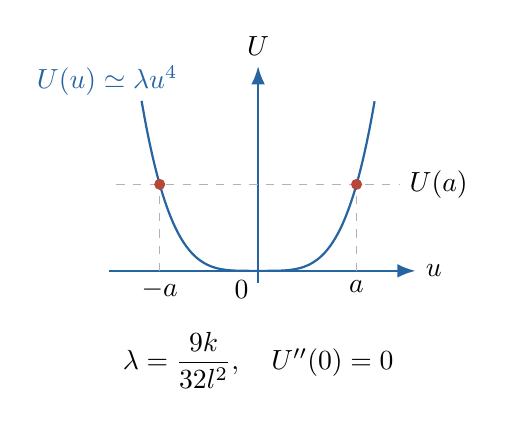
\begin{tikzpicture}
\draw[vec](-1.9,0)--(2,0)node[right]{$u$};
\draw[vec](0,-.15)--(0,2.6)node[above]{$U$};
\draw[blue,thick,domain=-1.48:1.48,samples=90]plot(\x,{.45*(\x)^4});
\draw[guide](-1.8,1.09863)--(1.8,1.09863);
\node[right]at(1.8,1.09863){$U(a)$};
\draw[guide](-1.25,0)--(-1.25,1.09863);
\draw[guide](1.25,0)--(1.25,1.09863);
\fill[red](-1.25,1.09863)circle(2pt);
\fill[red](1.25,1.09863)circle(2pt);
\node[below]at(-1.25,0){$-a$};\node[below]at(1.25,0){$a$};
\node[below left]at(0,0){$0$};
\node[blue,above left]at(-.9,2.1){$U(u)\simeq\lambda u^4$};
\node[below]at(0,-.65){$\lambda=\dfrac{9k}{32l^2},\quad U''(0)=0$};
\end{tikzpicture}
\end{document}
